\PassOptionsToPackage{table}{xcolor}
\documentclass[aspectratio=169,11pt]{beamer}

% ── Theme ─────────────────────────────────────────────────────────────────────
\usetheme{metropolis}
\usepackage{appendixnumberbeamer}

% ── Packages ──────────────────────────────────────────────────────────────────
\usepackage[utf8]{inputenc}
\usepackage[T1]{fontenc}
\usepackage{amsmath,amssymb}
\usepackage{booktabs}
\usepackage{graphicx}
\usepackage{algorithm}
\usepackage{algpseudocode}
\usepackage{listings}
\usepackage{xcolor}
\usepackage{tikz}
\usepackage{array}

\lstset{
  basicstyle=\ttfamily\scriptsize,
  breaklines=true,
  frame=none,
  backgroundcolor=\color{gray!10},
  keywordstyle=\color{blue!70!black},
  commentstyle=\color{green!50!black}\itshape,
  stringstyle=\color{red!60!black},
}

\newcommand{\pres}[2]{\langle #1 \mid #2 \rangle}
\newcommand{\inv}[1]{#1^{-1}}

% ── Colours ───────────────────────────────────────────────────────────────────
\definecolor{good}{HTML}{2E7D32}
\definecolor{bad}{HTML}{C62828}
\definecolor{accent}{HTML}{1565C0}
\definecolor{highlight}{HTML}{FFF9C4}

% ── Title ─────────────────────────────────────────────────────────────────────
\title{Reproducing Results on the\\Andrews--Curtis Conjecture}
\subtitle{Classical Search and PPO}
\author{AC-Solver Project}
\date{April 2026}

\begin{document}

% ══════════════════════════════════════════════════════════════════════════════
\maketitle

% ══════════════════════════════════════════════════════════════════════════════
\begin{frame}{Outline}
  \tableofcontents
\end{frame}

% ══════════════════════════════════════════════════════════════════════════════
\section{Introduction}
% ══════════════════════════════════════════════════════════════════════════════

% ──────────────────────────────────────────────────────────────────────────────
\begin{frame}{The Andrews--Curtis Conjecture}
  \begin{block}{Conjecture (Andrews \& Curtis, 1965)}
    Every balanced presentation of the trivial group can be reduced to $\pres{x,y}{x,y}$
    using a finite sequence of \textbf{AC moves}.
  \end{block}

  \bigskip

  Computationally, this is a \textbf{graph search problem}:
  \begin{itemize}
    \item \textbf{Node:} a balanced presentation $\pres{x,y}{r_0, r_1}$
    \item \textbf{Edge:} one of 12 AC moves
    \item \textbf{Goal:} reach a trivial node (total relator length $= 2$)
  \end{itemize}

  \bigskip
  \textcolor{gray}{Status: open for 60+ years despite extensive computational effort.}
\end{frame}

% ──────────────────────────────────────────────────────────────────────────────
\begin{frame}{The Miller--Schupp Dataset}
  Parameterised by integer $n \ge 1$ and a word $w$ in generators $\{x, \inv{x}, y, \inv{y}\}$
  with \textbf{zero exponent sum on $x$} (i.e.\ \#$x$ $=$ \#$\inv{x}$ in $w$):
  \[
    \mathrm{MS}(n, w) \;=\; \pres{x, y}{\underbrace{\inv{x}\, y^n\, x\, y^{-(n+1)}}_{r_0\text{: fixed by }n},\;\;
    \underbrace{\inv{x}\, w}_{r_1\text{: varies with }w}}
  \]

  \begin{itemize}
    \item $n$ controls the \textbf{complexity} of the first relator $r_0$
    \item $w$ is a \textbf{balanced word} that defines the second relator $r_1 = \inv{x}\, w$
    \item $n \in \{1, \ldots, 7\}$, $|w| \in \{1, \ldots, 7\}$; after removing cyclic
      permutations: \textbf{1190 presentations}
  \end{itemize}

  \medskip
  \textbf{Example 1} ($n{=}1$, $w{=}y$, $|w|{=}1$): instance \#0 in the dataset
  \[
    \pres{x,y}{\inv{x}\, y\, x\, y^{-2},\;\;\inv{x}\, y}
    \;\;\longleftrightarrow\;\;
    \texttt{[-1, 2, 1, -2, -2, 0,\ldots, -1, 2, 0,\ldots]}
  \]

  \textbf{Example 2} ($n{=}2$, $w{=}y$, $|w|{=}1$): instance \#170
  \[
    \pres{x,y}{\inv{x}\, y^2\, x\, y^{-3},\;\;\inv{x}\, y}
    \;\;\longleftrightarrow\;\;
    \texttt{[-1, 2, 2, 1, -2, -2, -2, 0,\ldots, -1, 2, 0,\ldots]}
  \]

  \smallskip
  \textbf{Solved} $=$ total relator length $= 2$ (e.g.\ $\pres{x,y}{x, \inv{y}}$).
\end{frame}

% ══════════════════════════════════════════════════════════════════════════════
\section{The 12 AC Moves}
% ══════════════════════════════════════════════════════════════════════════════

% ──────────────────────────────────────────────────────────────────────────────
\begin{frame}{The 12 AC Moves}
  \small
  \begin{columns}[T]
    \begin{column}{0.48\textwidth}
      \textbf{4 Concatenations}
      \begin{tabular}{cl}
        \toprule
        \textbf{ID} & \textbf{Operation} \\
        \midrule
        0 & $r_1 \leftarrow r_1 \cdot r_0$ \\
        1 & $r_0 \leftarrow r_0 \cdot \inv{r_1}$ \\
        2 & $r_1 \leftarrow r_1 \cdot \inv{r_0}$ \\
        3 & $r_0 \leftarrow r_0 \cdot r_1$ \\
        \bottomrule
      \end{tabular}
    \end{column}
    \begin{column}{0.48\textwidth}
      \textbf{8 Conjugations}
      \begin{tabular}{cl}
        \toprule
        \textbf{ID} & \textbf{Operation} \\
        \midrule
        4  & $r_1 \leftarrow \inv{x} \cdot r_1 \cdot x$ \\
        5  & $r_0 \leftarrow \inv{y} \cdot r_0 \cdot y$ \\
        6  & $r_1 \leftarrow \inv{y} \cdot r_1 \cdot y$ \\
        7  & $r_0 \leftarrow x \cdot r_0 \cdot \inv{x}$ \\
        8  & $r_1 \leftarrow x \cdot r_1 \cdot \inv{x}$ \\
        9  & $r_0 \leftarrow y \cdot r_0 \cdot \inv{y}$ \\
        10 & $r_1 \leftarrow y \cdot r_1 \cdot \inv{y}$ \\
        11 & $r_0 \leftarrow \inv{x} \cdot r_0 \cdot x$ \\
        \bottomrule
      \end{tabular}
    \end{column}
  \end{columns}

  \bigskip
  \begin{itemize}
    \item \textbf{Free reduction} applied after every move ($x \cdot \inv{x} \to \epsilon$)
    \item Move \textbf{rejected} if result exceeds \texttt{max\_relator\_length}~$= 36$ (no-op)
    \item $\sim$69\% of PPO actions are no-ops
  \end{itemize}
\end{frame}

% ══════════════════════════════════════════════════════════════════════════════
\section{Classical Search}
% ══════════════════════════════════════════════════════════════════════════════

% ──────────────────────────────────────────────────────────────────────────────
\begin{frame}{Greedy Search}
  \textbf{Core idea:} always expand the state with the \alert{shortest total length}.

  \begin{columns}[T]
    \begin{column}{0.55\textwidth}
      \textbf{Algorithm:}
      \begin{enumerate}
        \item Push initial state onto a \textbf{min-heap}\\
              (priority $=$ total relator length)
        \item Pop shortest state; try all 12 moves
        \item If new length $= 2$: \textcolor{good}{solved!}
        \item If unseen: push onto heap
        \item Repeat until solved or node budget exhausted
      \end{enumerate}
    \end{column}
    \begin{column}{0.42\textwidth}
      \textbf{Properties:}
      \begin{itemize}
        \item[\textcolor{good}{\checkmark}] Fast (explores fewer nodes)
        \item[\textcolor{bad}{$\times$}] No shortest-path guarantee
        \item Tie-break: path length, then lexicographic
        \item Cost: $O(\log n)$ per step
      \end{itemize}
    \end{column}
  \end{columns}

  \bigskip
  \footnotesize\texttt{ac\_solver/search/greedy.py}
\end{frame}

% ──────────────────────────────────────────────────────────────────────────────
\begin{frame}{Breadth-First Search (BFS)}
  \textbf{Core idea:} expand states \alert{level by level} (all depth $d$ before $d{+}1$).

  \begin{columns}[T]
    \begin{column}{0.55\textwidth}
      \textbf{Algorithm:}
      \begin{enumerate}
        \item Push initial state onto a \textbf{FIFO queue}
        \item Pop oldest state; try all 12 moves
        \item If new length $= 2$: \textcolor{good}{solved!}\\
              (guaranteed shortest path)
        \item If unseen: append to back of queue
        \item Repeat until solved or node budget exhausted
      \end{enumerate}
    \end{column}
    \begin{column}{0.42\textwidth}
      \textbf{Properties:}
      \begin{itemize}
        \item[\textcolor{good}{\checkmark}] \textbf{Shortest-path guarantee}
        \item[\textcolor{bad}{$\times$}] Slower (exhaustive per level)
        \item Cost: $O(1)$ per step
      \end{itemize}

      \bigskip
      \textit{First solution found is always optimal (fewest AC moves).}
    \end{column}
  \end{columns}

  \bigskip
  \footnotesize\texttt{ac\_solver/search/breadth\_first.py}
\end{frame}

% ──────────────────────────────────────────────────────────────────────────────
\begin{frame}{Greedy vs.\ BFS}
  \begin{center}
  \begin{tabular}{lll}
    \toprule
    \textbf{Aspect} & \textbf{Greedy} & \textbf{BFS} \\
    \midrule
    Data structure   & Min-heap          & FIFO deque \\
    Expansion order  & Shortest length first & By depth \\
    Shortest path?   & \textcolor{bad}{No}  & \textcolor{good}{Yes} \\
    Typical speed    & \textcolor{good}{Faster} & Slower \\
    Per-step cost    & $O(\log n)$       & $O(1)$ \\
    \bottomrule
  \end{tabular}
  \end{center}

  \bigskip
  \textbf{Trade-off:} Greedy is biased toward short states (fast, approximate).
  BFS is unbiased (slow, optimal).
\end{frame}

% ──────────────────────────────────────────────────────────────────────────────
\begin{frame}{Classical Search Pipeline: No Training Required}
  \textbf{Dataset:} all 1190 Miller--Schupp presentations ($n \in [1,7]$, $|w| \in [1,7]$).

  \bigskip
  \begin{columns}[T]
    \begin{column}{0.48\textwidth}
      \textbf{Classical (Greedy / BFS):}
      \begin{enumerate}
        \item Load dataset (1190 presentations)
        \item For each: run search ($\le 10^6$ nodes)
        \item Record solved / path / time to CSV
        \item \textcolor{good}{No model, no training, no GPU}
      \end{enumerate}
      \smallskip
      {\footnotesize Multiprocessing + resumable CSV.\\
      Wall-clock: $\sim$2\,h (greedy) / $\sim$6\,h (BFS).}
    \end{column}
    \begin{column}{0.48\textwidth}
      \textbf{PPO (contrast):}
      \begin{enumerate}
        \item Load dataset
        \item \alert{Train policy for $10^8$ steps ($\sim$60\,h)}
        \item Load best checkpoint
        \item Evaluate on all presentations
      \end{enumerate}
      \smallskip
      {\footnotesize Requires GPU/MPS, hyperparameter tuning,\\
      and careful reward engineering.}
    \end{column}
  \end{columns}

  \bigskip
  \footnotesize\texttt{ac\_solver/search/miller\_schupp/evaluate.py}
\end{frame}

% ──────────────────────────────────────────────────────────────────────────────
\begin{frame}[fragile]{Classical Search Results}
  \begin{center}
  \begin{tabular}{lrrr}
    \toprule
    \textbf{Algorithm} & \textbf{Solved} & \textbf{Solve Rate} & \textbf{Paper} \\
    \midrule
    Greedy ($10^6$ nodes) & \textbf{554} / 1190 & \textbf{46.6\%} & 533 (44.8\%) \\
    BFS ($10^6$ nodes)    & 278 / 1190           & 23.4\%           & 278 (23.4\%) \\
    \bottomrule
  \end{tabular}
  \end{center}

  \begin{itemize}
    \item BFS matches the paper \textbf{exactly}
    \item Greedy: +21 instances (minor tie-breaking differences)
  \end{itemize}

  \bigskip
  \textbf{Reproduce:}
  \begin{lstlisting}[language=bash]
python -m ac_solver.search.miller_schupp.evaluate \
    --search-fn greedy --max-nodes 1000000 --workers 4 --full
python -m ac_solver.search.miller_schupp.evaluate \
    --search-fn bfs --max-nodes 1000000 --workers 4 --full
  \end{lstlisting}
\end{frame}

% ──────────────────────────────────────────────────────────────────────────────
\begin{frame}{Results by Difficulty: Solve Rate}
  \vspace{-0.5em}
  \begin{center}
    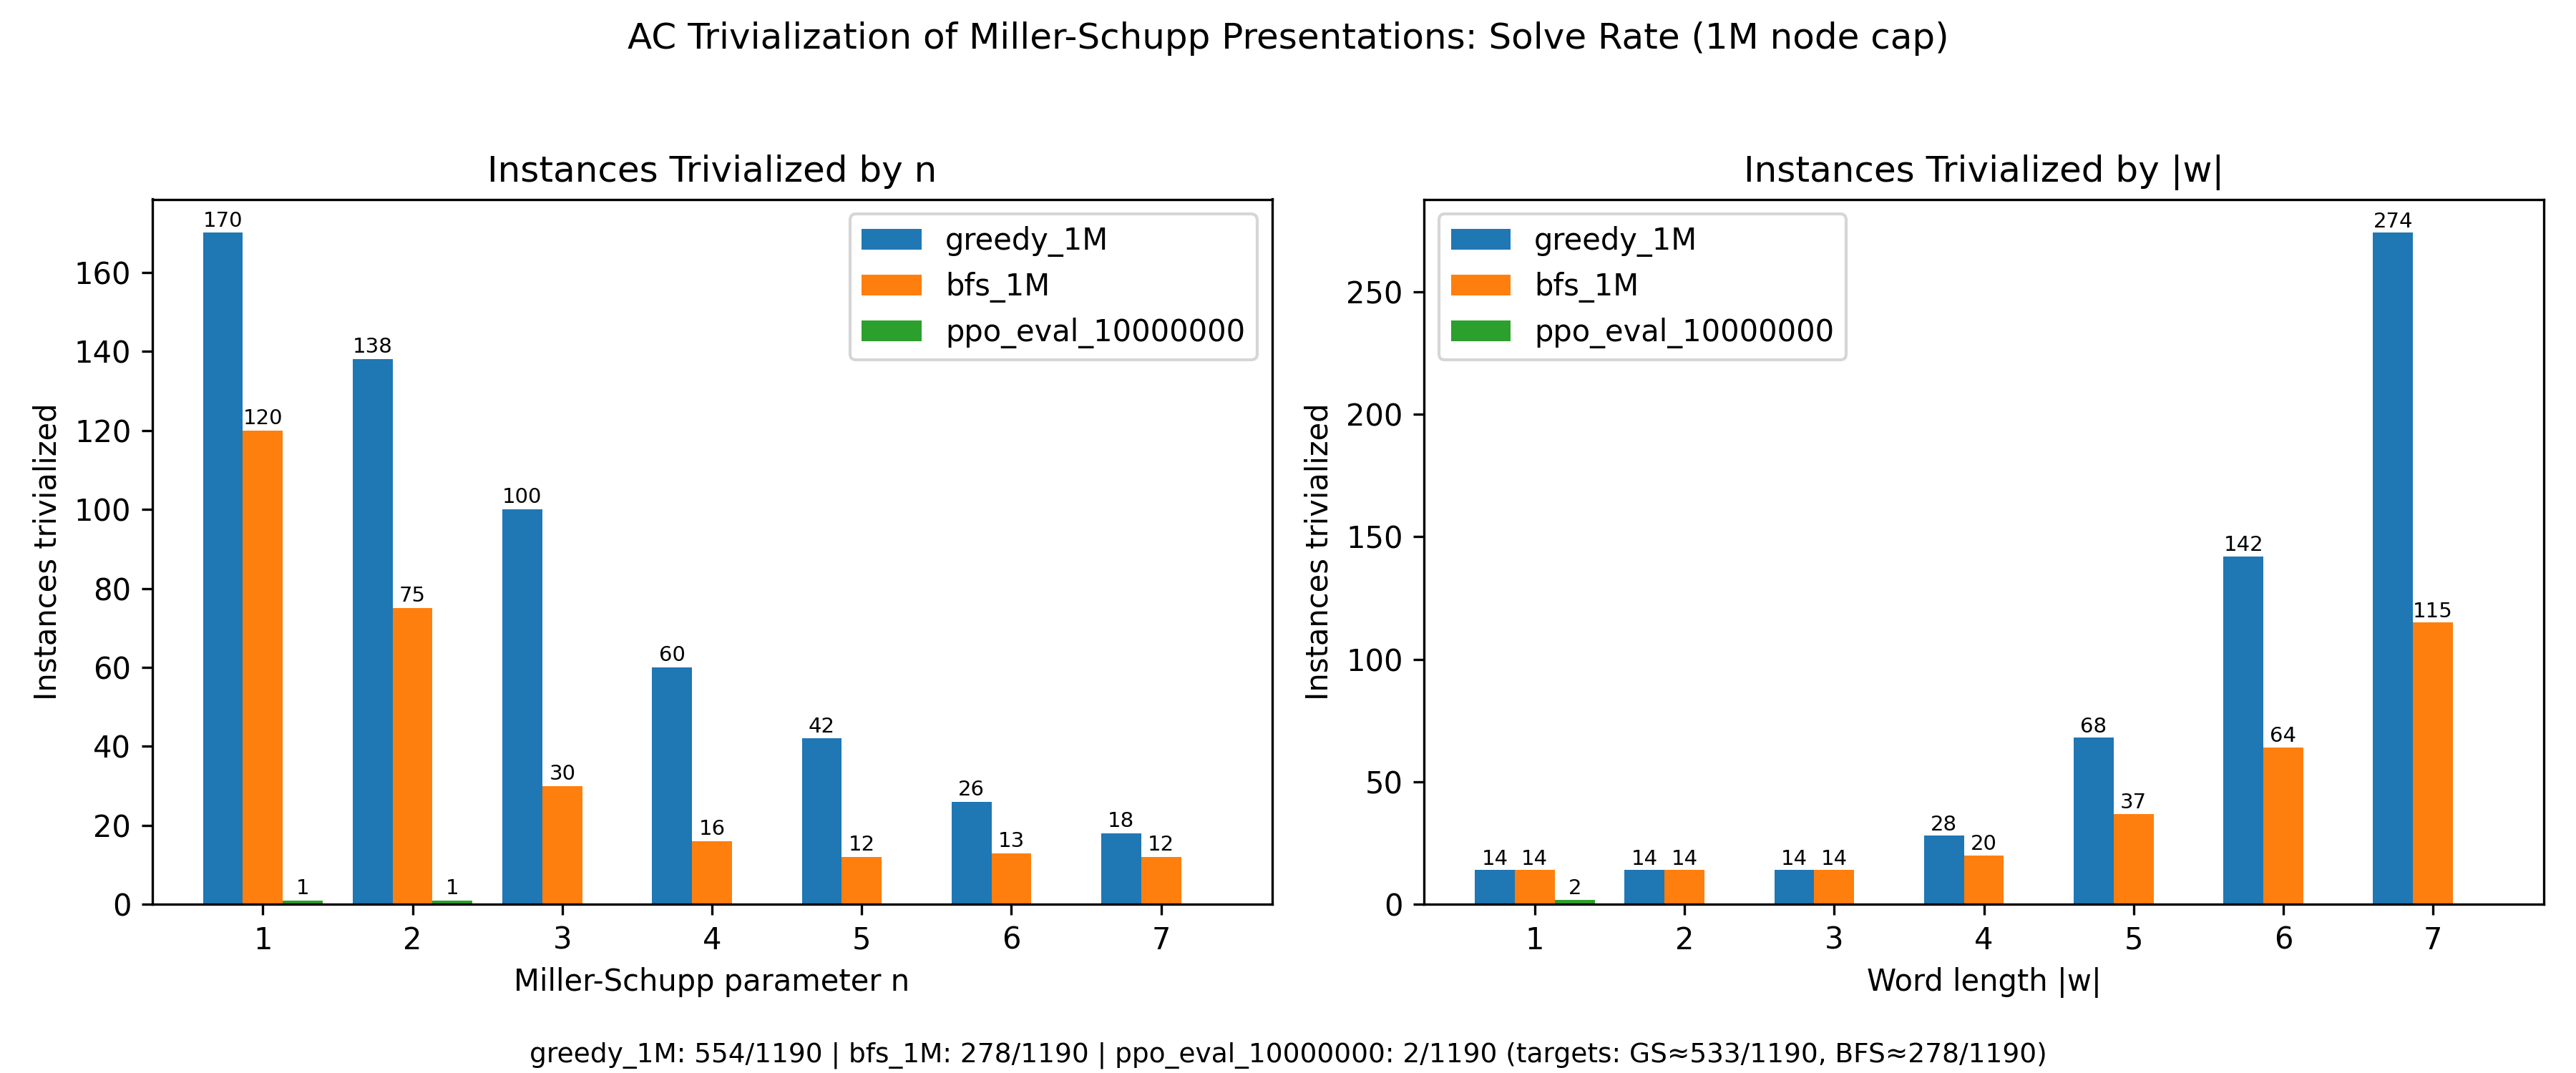
\includegraphics[width=0.73\textwidth]{figures/ac_trivialization_solve_rate.png}
  \end{center}
  \vspace{-0.8em}
  \footnotesize
  \begin{itemize}\setlength\itemsep{1pt}
    \item \textbf{Left:} solved vs.\ $n$.  Higher $n$ $\Rightarrow$ longer $r_0$ $\Rightarrow$ larger search space.  Both greedy and BFS degrade sharply.
    \item \textbf{Right:} solved vs.\ $|w|$.  Weaker effect---greedy solves \emph{more} at high $|w|$ (free-reduction opportunities).
    \item \textbf{PPO} (green) solves almost nothing at any difficulty level.
  \end{itemize}
\end{frame}

% ──────────────────────────────────────────────────────────────────────────────
\begin{frame}{Results by Difficulty: Heatmap}
  \begin{center}
    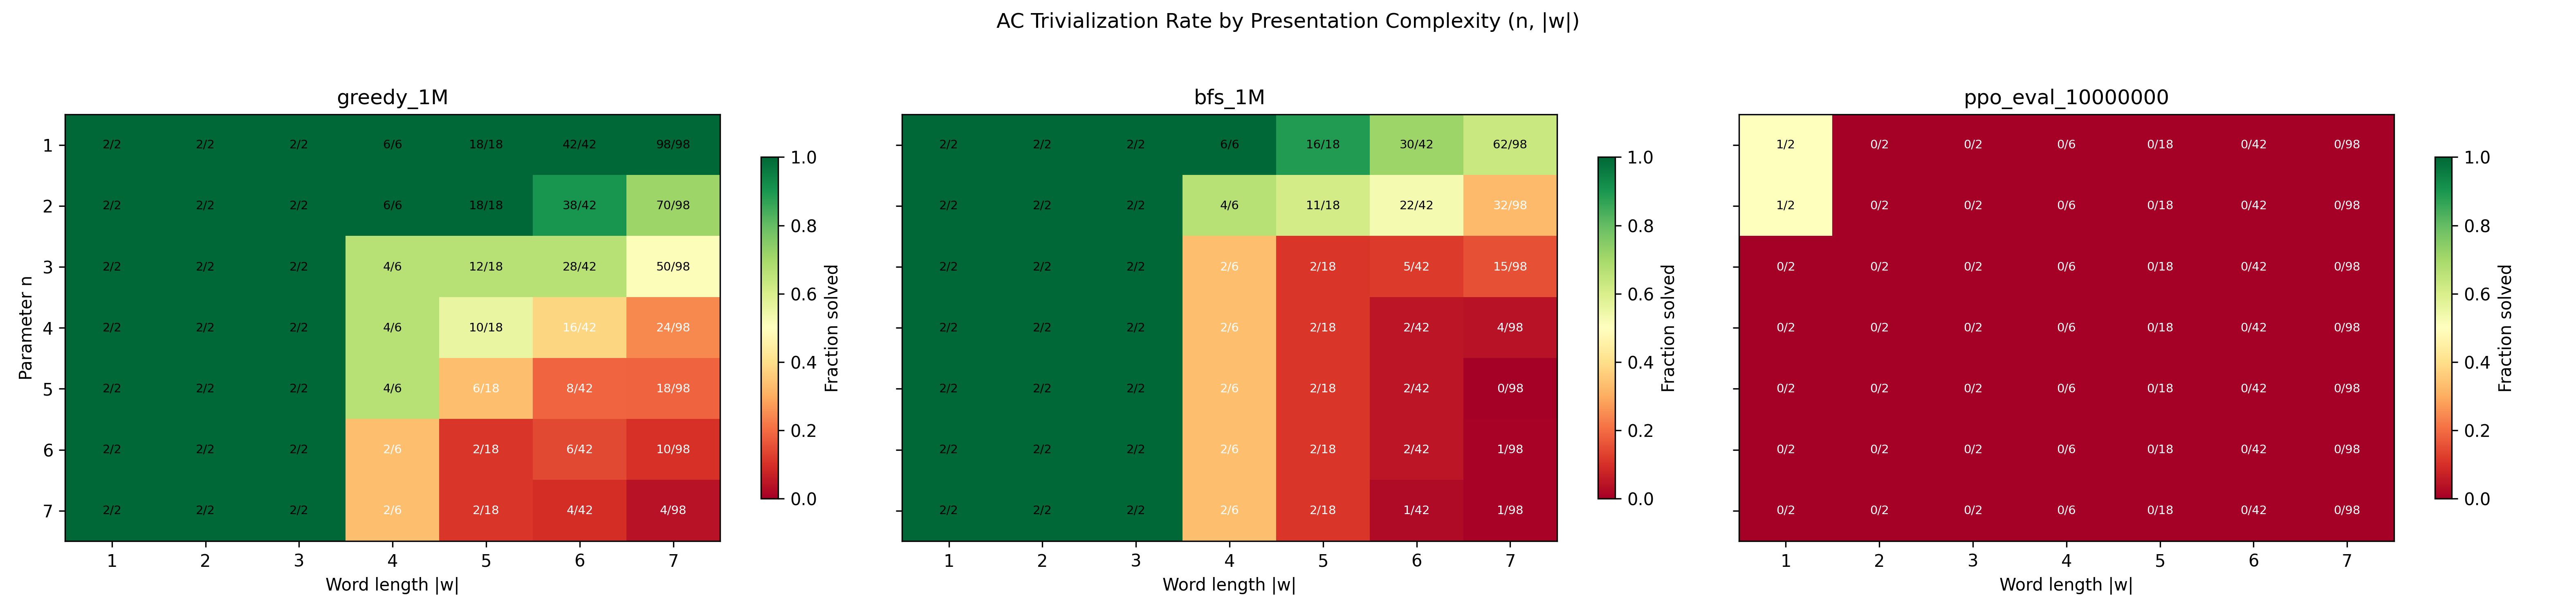
\includegraphics[width=0.95\textwidth]{figures/ac_trivialization_heatmap_n_vs_w.png}
  \end{center}
  \vspace{-0.5em}
  \small
  Three heatmaps showing solve rate for each $(n, |w|)$ cell (green $=$ high, red $=$ low):
  \begin{itemize}
    \item \textbf{Greedy (left):} strong at low $n$ (top rows), degrades toward
      bottom-left (high $n$, short $w$).
    \item \textbf{BFS (centre):} similar pattern but solves fewer cells overall;
      its exhaustive search hits the $10^6$-node budget sooner.
    \item \textbf{PPO (right):} almost entirely red---the policy cannot solve any
      cell reliably.
  \end{itemize}
\end{frame}

% ──────────────────────────────────────────────────────────────────────────────
\begin{frame}{Path Lengths and Length Increase}
  \begin{center}
    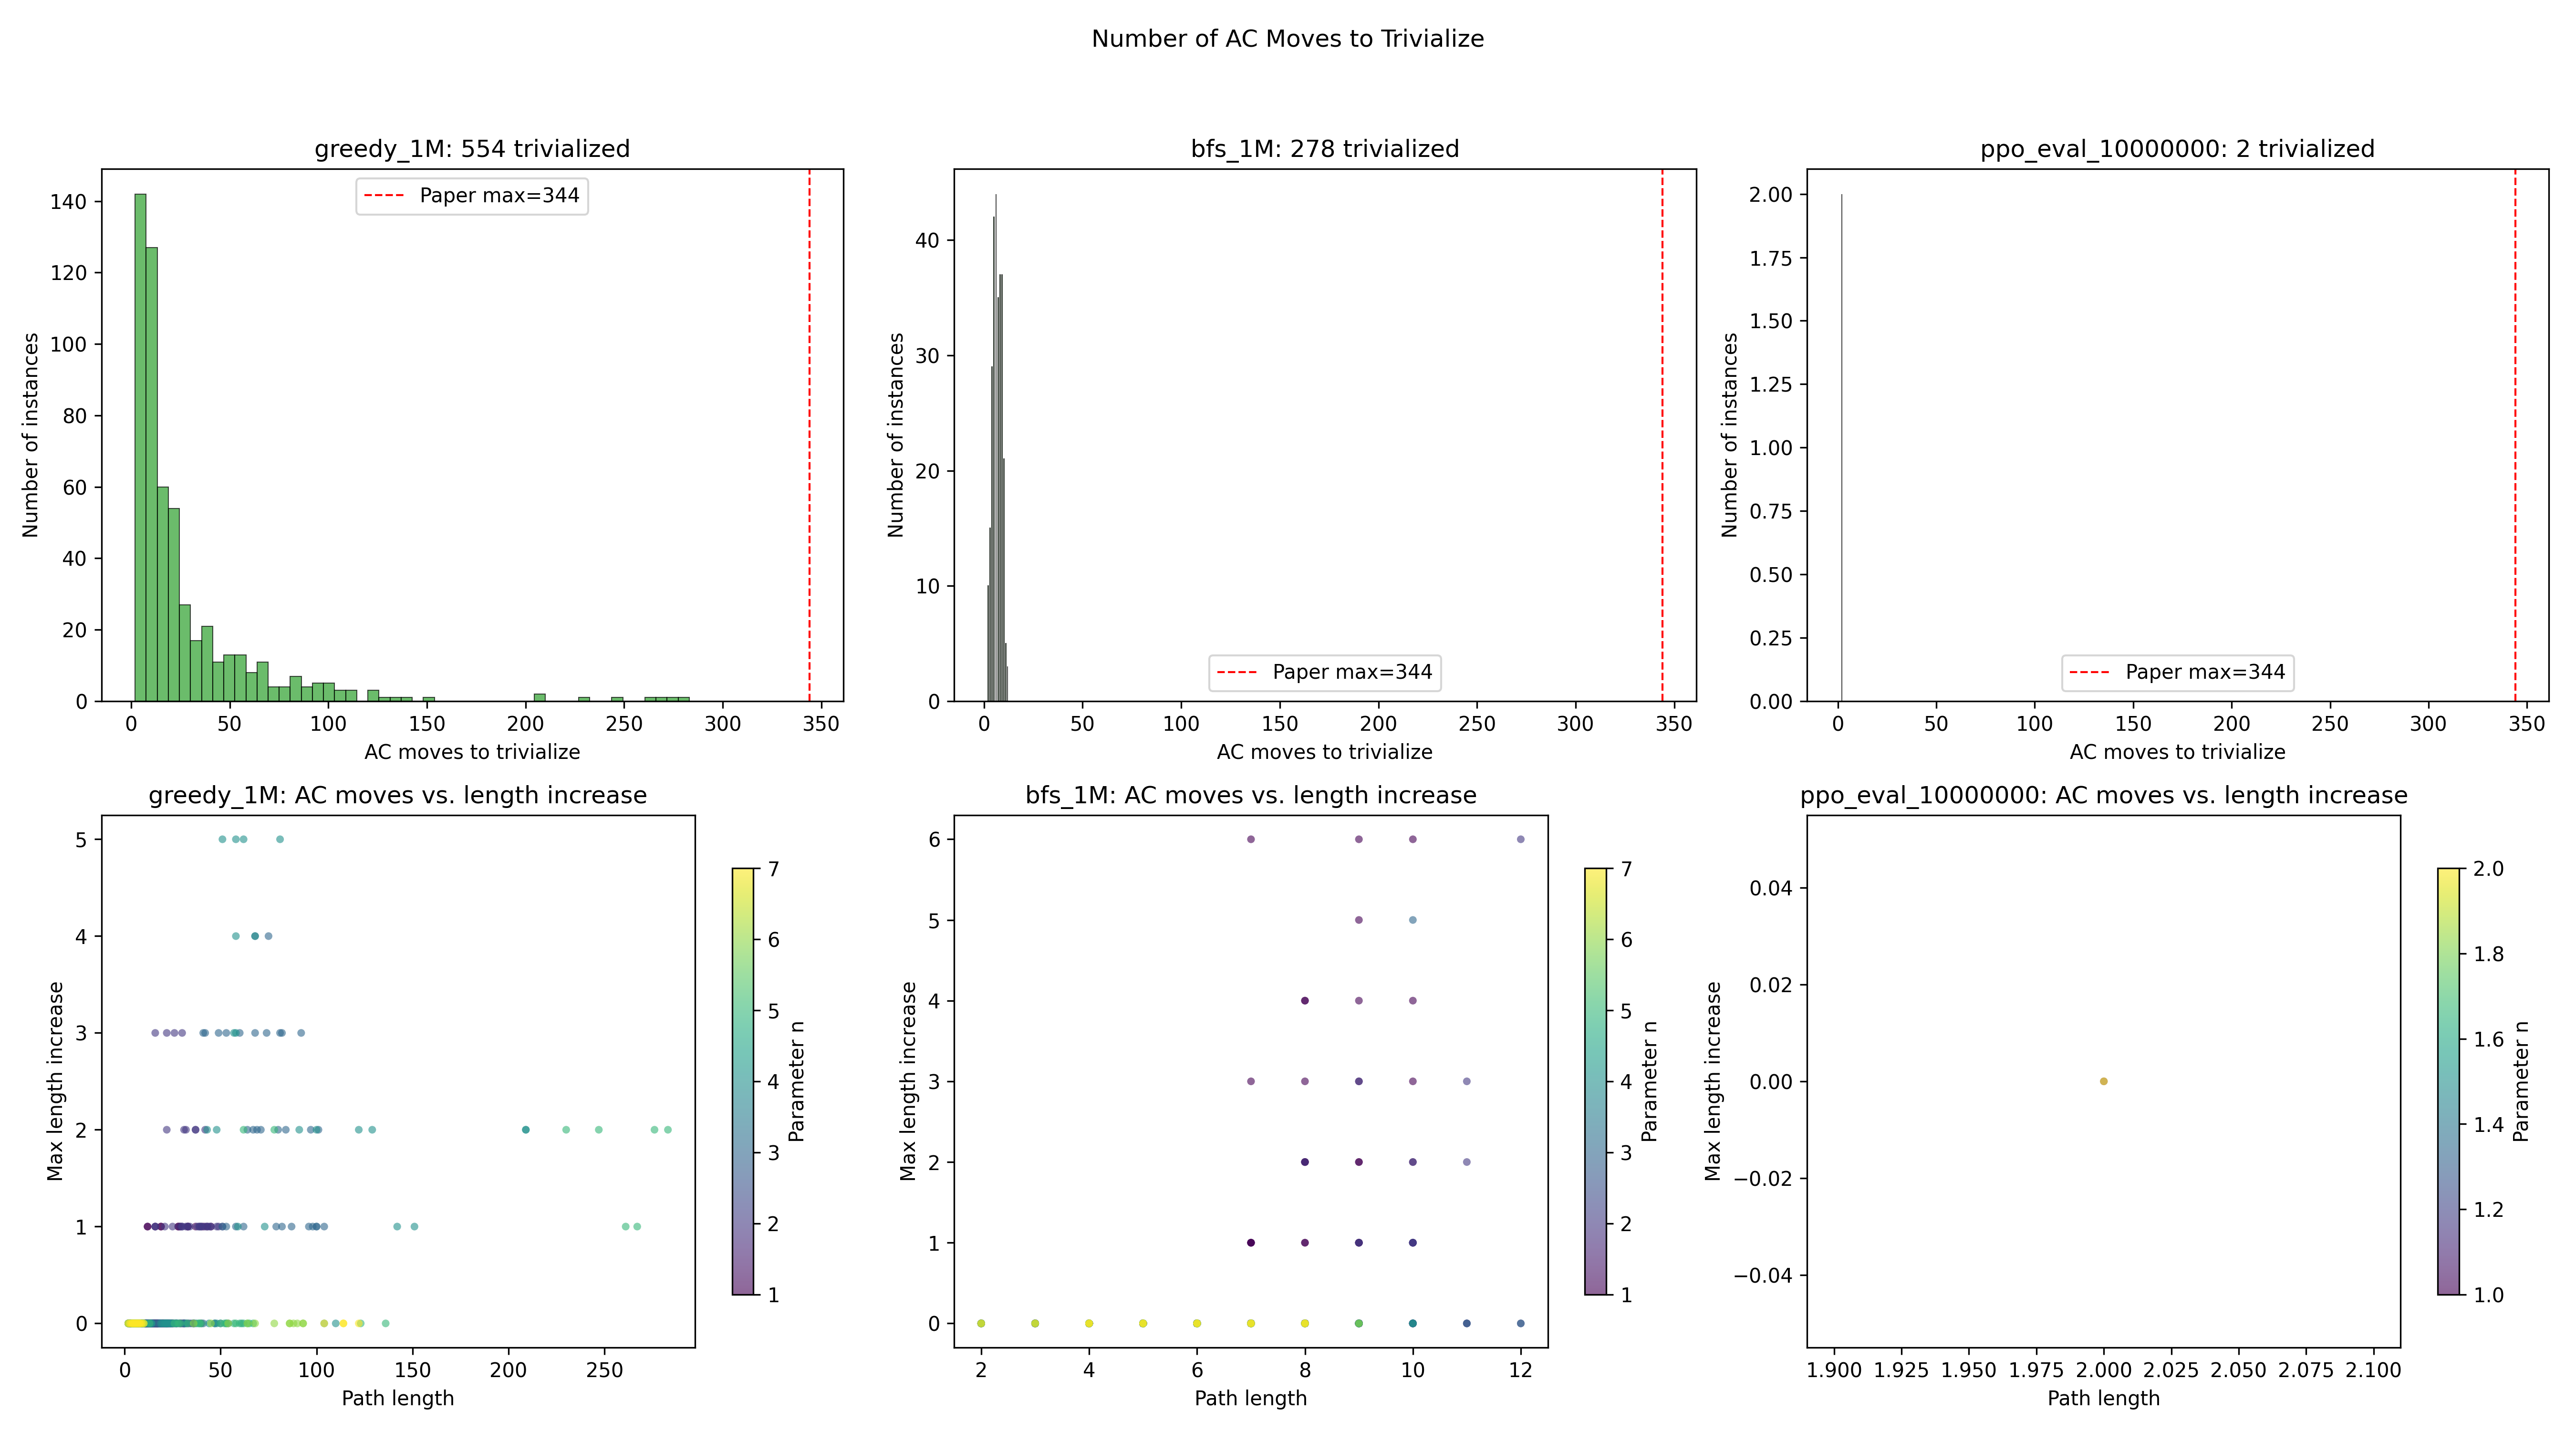
\includegraphics[width=0.92\textwidth]{figures/ac_path_steps_to_trivialization.png}
  \end{center}
  \vspace{-0.5em}
  \small
  \begin{itemize}
    \item \textbf{Top row:} histograms of solution path length (number of AC moves).
      Greedy (554 solved) has a long tail up to $\sim$250 moves; BFS (278 solved) peaks
      earlier because it finds the \emph{shortest} paths.  PPO solved only 2 here.
    \item \textbf{Bottom row:} path length vs.\ max length increase (peak relator
      length $-$ initial length during the solution path).  BFS solutions cluster
      near zero increase; greedy solutions sometimes inflate relators significantly
      before reducing them---a trade-off of its heuristic ordering.
  \end{itemize}
\end{frame}

% ══════════════════════════════════════════════════════════════════════════════
\section{PPO Reproduction}
% ══════════════════════════════════════════════════════════════════════════════

% ──────────────────────────────────────────────────────────────────────────────
\begin{frame}{PPO Agent Architecture}
  \begin{center}
  \begin{tabular}{lll}
    \toprule
    \textbf{Network} & \textbf{Architecture} & \textbf{Init} \\
    \midrule
    Actor  & $72 \to 512 \to 512 \to 12$ (Tanh) & Ortho ($\sqrt{2}$ / $0.01$) \\
    Critic & $72 \to 512 \to 512 \to 1$ (Tanh)  & Ortho ($\sqrt{2}$ / $1.0$) \\
    \bottomrule
  \end{tabular}
  \end{center}

  \bigskip
  \begin{itemize}
    \item \textbf{Input:} 72 $= 2 \times 36$ (two relators, zero-padded)
    \item \textbf{Output:} 12 logits $\to$ $\mathrm{Categorical}$ (training) / $\arg\max$ (eval)
    \item Separate actor and critic (no shared layers)
    \item Actor output init $= 0.01$ $\Rightarrow$ near-uniform initial policy
  \end{itemize}
\end{frame}

% ──────────────────────────────────────────────────────────────────────────────
\begin{frame}{Hyperparameters: Paper vs.\ Mac Reproduction}
  \small
  \begin{center}
  \begin{tabular}{lrrl}
    \toprule
    \textbf{Parameter} & \textbf{Paper} & \textbf{Mac} & \textbf{Notes} \\
    \midrule
    \texttt{total\_timesteps} & $10^8$ & $10^8$ & Same \\
    \texttt{num\_envs}        & 28     & \alert{8} & Hardware \\
    \texttt{batch\_size}      & 5{,}600 & \alert{1{,}600} & $3.5\times$ smaller \\
    \texttt{update\_epochs}   & 1      & 1      & Single pass \\
    \texttt{learning\_rate}   & \multicolumn{2}{c}{$10^{-4} \to 0$} & Linear decay \\
    $\gamma$                  & 0.999  & 0.999  & \\
    $\epsilon_\text{clip}$    & 0.2    & 0.2    & \\
    $c_\text{ent}$            & 0.01   & 0.01   & \\
    \midrule
    \textbf{PPO updates}      & 17{,}857 & \alert{62{,}500} & $3.5\times$ more \\
    \bottomrule
  \end{tabular}
  \end{center}

  \bigskip
  $3.5\times$ more updates, but each with $3.5\times$ noisier batch.
\end{frame}

% ──────────────────────────────────────────────────────────────────────────────
\begin{frame}{Paper vs.\ Reproduction: What Matches, What Doesn't}
  \small
  \begin{center}
  \begin{tabular}{l@{\hskip 6pt}c@{\hskip 6pt}c@{\hskip 6pt}c}
    \toprule
    \textbf{Aspect} & \textbf{Paper} & \textbf{Our Repro} & \textbf{Match?} \\
    \midrule
    Network           & $[512, 512]$ MLP, Tanh     & Same              & \textcolor{good}{\checkmark} \\
    Separate actor/critic & Yes                     & Yes               & \textcolor{good}{\checkmark} \\
    Weight init       & Orthogonal                  & Orthogonal        & \textcolor{good}{\checkmark} \\
    LR schedule       & $10^{-4} \to 0$ linear      & Same              & \textcolor{good}{\checkmark} \\
    PPO hyperparams   & Table 1 (Appendix A)        & All identical     & \textcolor{good}{\checkmark} \\
    Adam $\epsilon$   & $10^{-5}$                   & $10^{-5}$         & \textcolor{good}{\checkmark} \\
    Curriculum        & $\frac{1}{4}$ solved, $\frac{3}{4}$ unsolved & Same & \textcolor{good}{\checkmark} \\
    AC moves          & 12 (AC'1 + AC'2)            & 12 (same set)     & \textcolor{good}{\checkmark} \\
    \texttt{max\_relator\_length} & 36               & 36                & \textcolor{good}{\checkmark} \\
    \midrule
    Parallel actors   & 28                          & \alert{8}         & \textcolor{bad}{$\times$} \\
    Batch size        & 5{,}600                     & \alert{1{,}600}   & \textcolor{bad}{$\times$} \\
    Reward normalisation & \textbf{None}            & \alert{$\div 14{,}400$} & \textcolor{bad}{$\times$} \\
    Variable horizon  & Yes (200$\to$1200)          & \alert{No (200 only)} & \textcolor{bad}{$\times$} \\
    \midrule
    \textbf{PPO solved}& \textbf{431/1190 (36.2\%)} & \textbf{32/1190 (2.7\%)} & \textcolor{bad}{$\mathbf{13\times}$ gap} \\
    \bottomrule
  \end{tabular}
  \end{center}
\end{frame}

% ──────────────────────────────────────────────────────────────────────────────
\begin{frame}{The Reward Mismatch: Smoking Gun}
  The paper defines the reward function \textbf{directly} (Section~4.3):
  \[
    R(s_t, a_t, s_{t+1}) = \begin{cases}
      -\min(10,\; \mathrm{length}(s_{t+1})) & \text{if } \mathrm{length}(s_{t+1}) > 2 \\
      +1000 & \text{otherwise (solved)}
    \end{cases}
  \]

  \textbf{No further normalisation is applied.}  The PPO update sees rewards in $[-10, +1000]$.

  \bigskip
  \textbf{Our code} adds an extra step \alert{not present in the paper}:
  \[
    \text{rewards} \;\mathrel{/}= \;\texttt{max\_reward} = 14{,}400
    \qquad\Longrightarrow\qquad
    \text{rewards} \in [-0.0007,\; +0.069]
  \]

  \begin{center}
    \begin{tabular}{lrr}
      \toprule
      & \textbf{Paper} & \textbf{Our code} \\
      \midrule
      Success reward seen by PPO & $+1000$ & $+0.069$ \\
      Per-step penalty           & $-10$   & $-0.0007$ \\
      \textbf{Signal-to-noise}   & \textcolor{good}{High} & \textcolor{bad}{$14{,}400\times$ weaker} \\
      \bottomrule
    \end{tabular}
  \end{center}

  \smallskip
  This single line (\texttt{training.py:332}) likely explains most of the $13\times$ performance gap.
\end{frame}

% ──────────────────────────────────────────────────────────────────────────────
\begin{frame}{Other Differences and What May Be Missing}
  \begin{columns}[T]
    \begin{column}{0.48\textwidth}
      \textbf{Batch size ($3.5\times$ smaller)}
      \begin{itemize}\small
        \item 8 envs $\times$ 200 steps $=$ 1{,}600
        \item Paper: 28 $\times$ 200 $=$ 5{,}600
        \item Noisier gradient estimates
        \item Fewer diverse presentations per batch
        \item Partially compensated by $3.5\times$ more updates
      \end{itemize}
    \end{column}
    \begin{column}{0.48\textwidth}
      \textbf{Variable horizon (not reproduced)}
      \begin{itemize}\small
        \item Paper: $T = 200 \to 400 \to 800 \to 1200$
        \item Increased at 10M, 25M, 50M steps
        \item Solved 2 new presentations greedy couldn't
        \item We only used constant $T = 200$
        \item Limits ability to solve long-path instances
      \end{itemize}
    \end{column}
  \end{columns}

  \bigskip
  \begin{block}{Priority Fix List}
    \begin{enumerate}\small
      \item \textbf{Remove} \texttt{rewards /= max\_reward} --- restore paper's reward scale
      \item \textbf{Increase} \texttt{num\_envs} to 28 (or max hardware allows)
      \item \textbf{Implement} variable horizon schedule
    \end{enumerate}
  \end{block}
\end{frame}

% ──────────────────────────────────────────────────────────────────────────────
\begin{frame}{Reward Pipeline: The $200\times$ Attenuation Problem}
  \begin{center}
  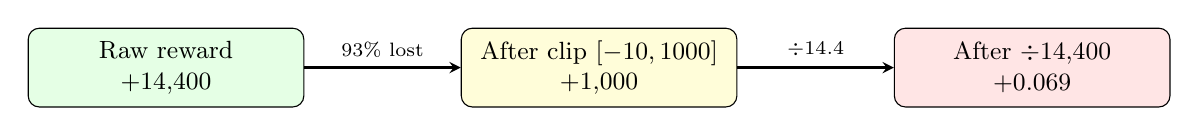
\begin{tikzpicture}[
    box/.style={draw, rounded corners, minimum height=1cm, minimum width=3.5cm,
                align=center, font=\small},
    arrow/.style={->, thick, >=stealth}
  ]
    \node[box, fill=green!10] (raw) at (0,0) {Raw reward\\$+14{,}400$};
    \node[box, fill=yellow!15] (clip) at (5.5,0) {After clip $[-10, 1000]$\\$+1{,}000$};
    \node[box, fill=red!10] (div) at (11,0) {After $\div 14{,}400$\\$+0.069$};

    \draw[arrow] (raw) -- node[above, font=\scriptsize] {93\% lost} (clip);
    \draw[arrow] (clip) -- node[above, font=\scriptsize] {$\div 14.4$} (div);
  \end{tikzpicture}
  \end{center}

  \bigskip
  \begin{itemize}
    \item \textbf{Raw success:} $+14{,}400$ ($= 200 \times 36 \times 2$)
    \item \textbf{Clipped:} $+1{,}000$ \quad $\Rightarrow$ \textcolor{bad}{93\% of signal discarded}
    \item \textbf{Normalised:} $+0.069$ \quad $\Rightarrow$ \textcolor{bad}{near noise level}
    \item Per-step penalty: $-0.00069$
  \end{itemize}

  \bigskip
  \alert{This is the single biggest issue} with the current training setup.
\end{frame}

% ──────────────────────────────────────────────────────────────────────────────
\begin{frame}{Training Execution}
  \begin{center}
  \begin{tabular}{lrrl}
    \toprule
    \textbf{Phase} & \textbf{Steps} & \textbf{Updates} & \textbf{Duration} \\
    \midrule
    Initial & $0 \to 38.8$M & $1 \to 24{,}285$ & $\sim$24 h \\
    Resumed & $38.7$M $\to$ $100$M & $24{,}201 \to 62{,}500$ & $\sim$36 h \\
    \midrule
    \textbf{Total} & $\mathbf{10^8}$ & \textbf{62{,}500} & $\sim$\textbf{60 h} \\
    \bottomrule
  \end{tabular}
  \end{center}

  \bigskip
  Checkpoints saved at: 1M, 5M, 10M, 20M, 50M, 100M steps.

  \bigskip
  \textbf{Curriculum:} cycle through 1190 presentations, then revisit solved with $p = 0.25$.
\end{frame}

% ──────────────────────────────────────────────────────────────────────────────
\begin{frame}{Training Curves}
  \begin{center}
    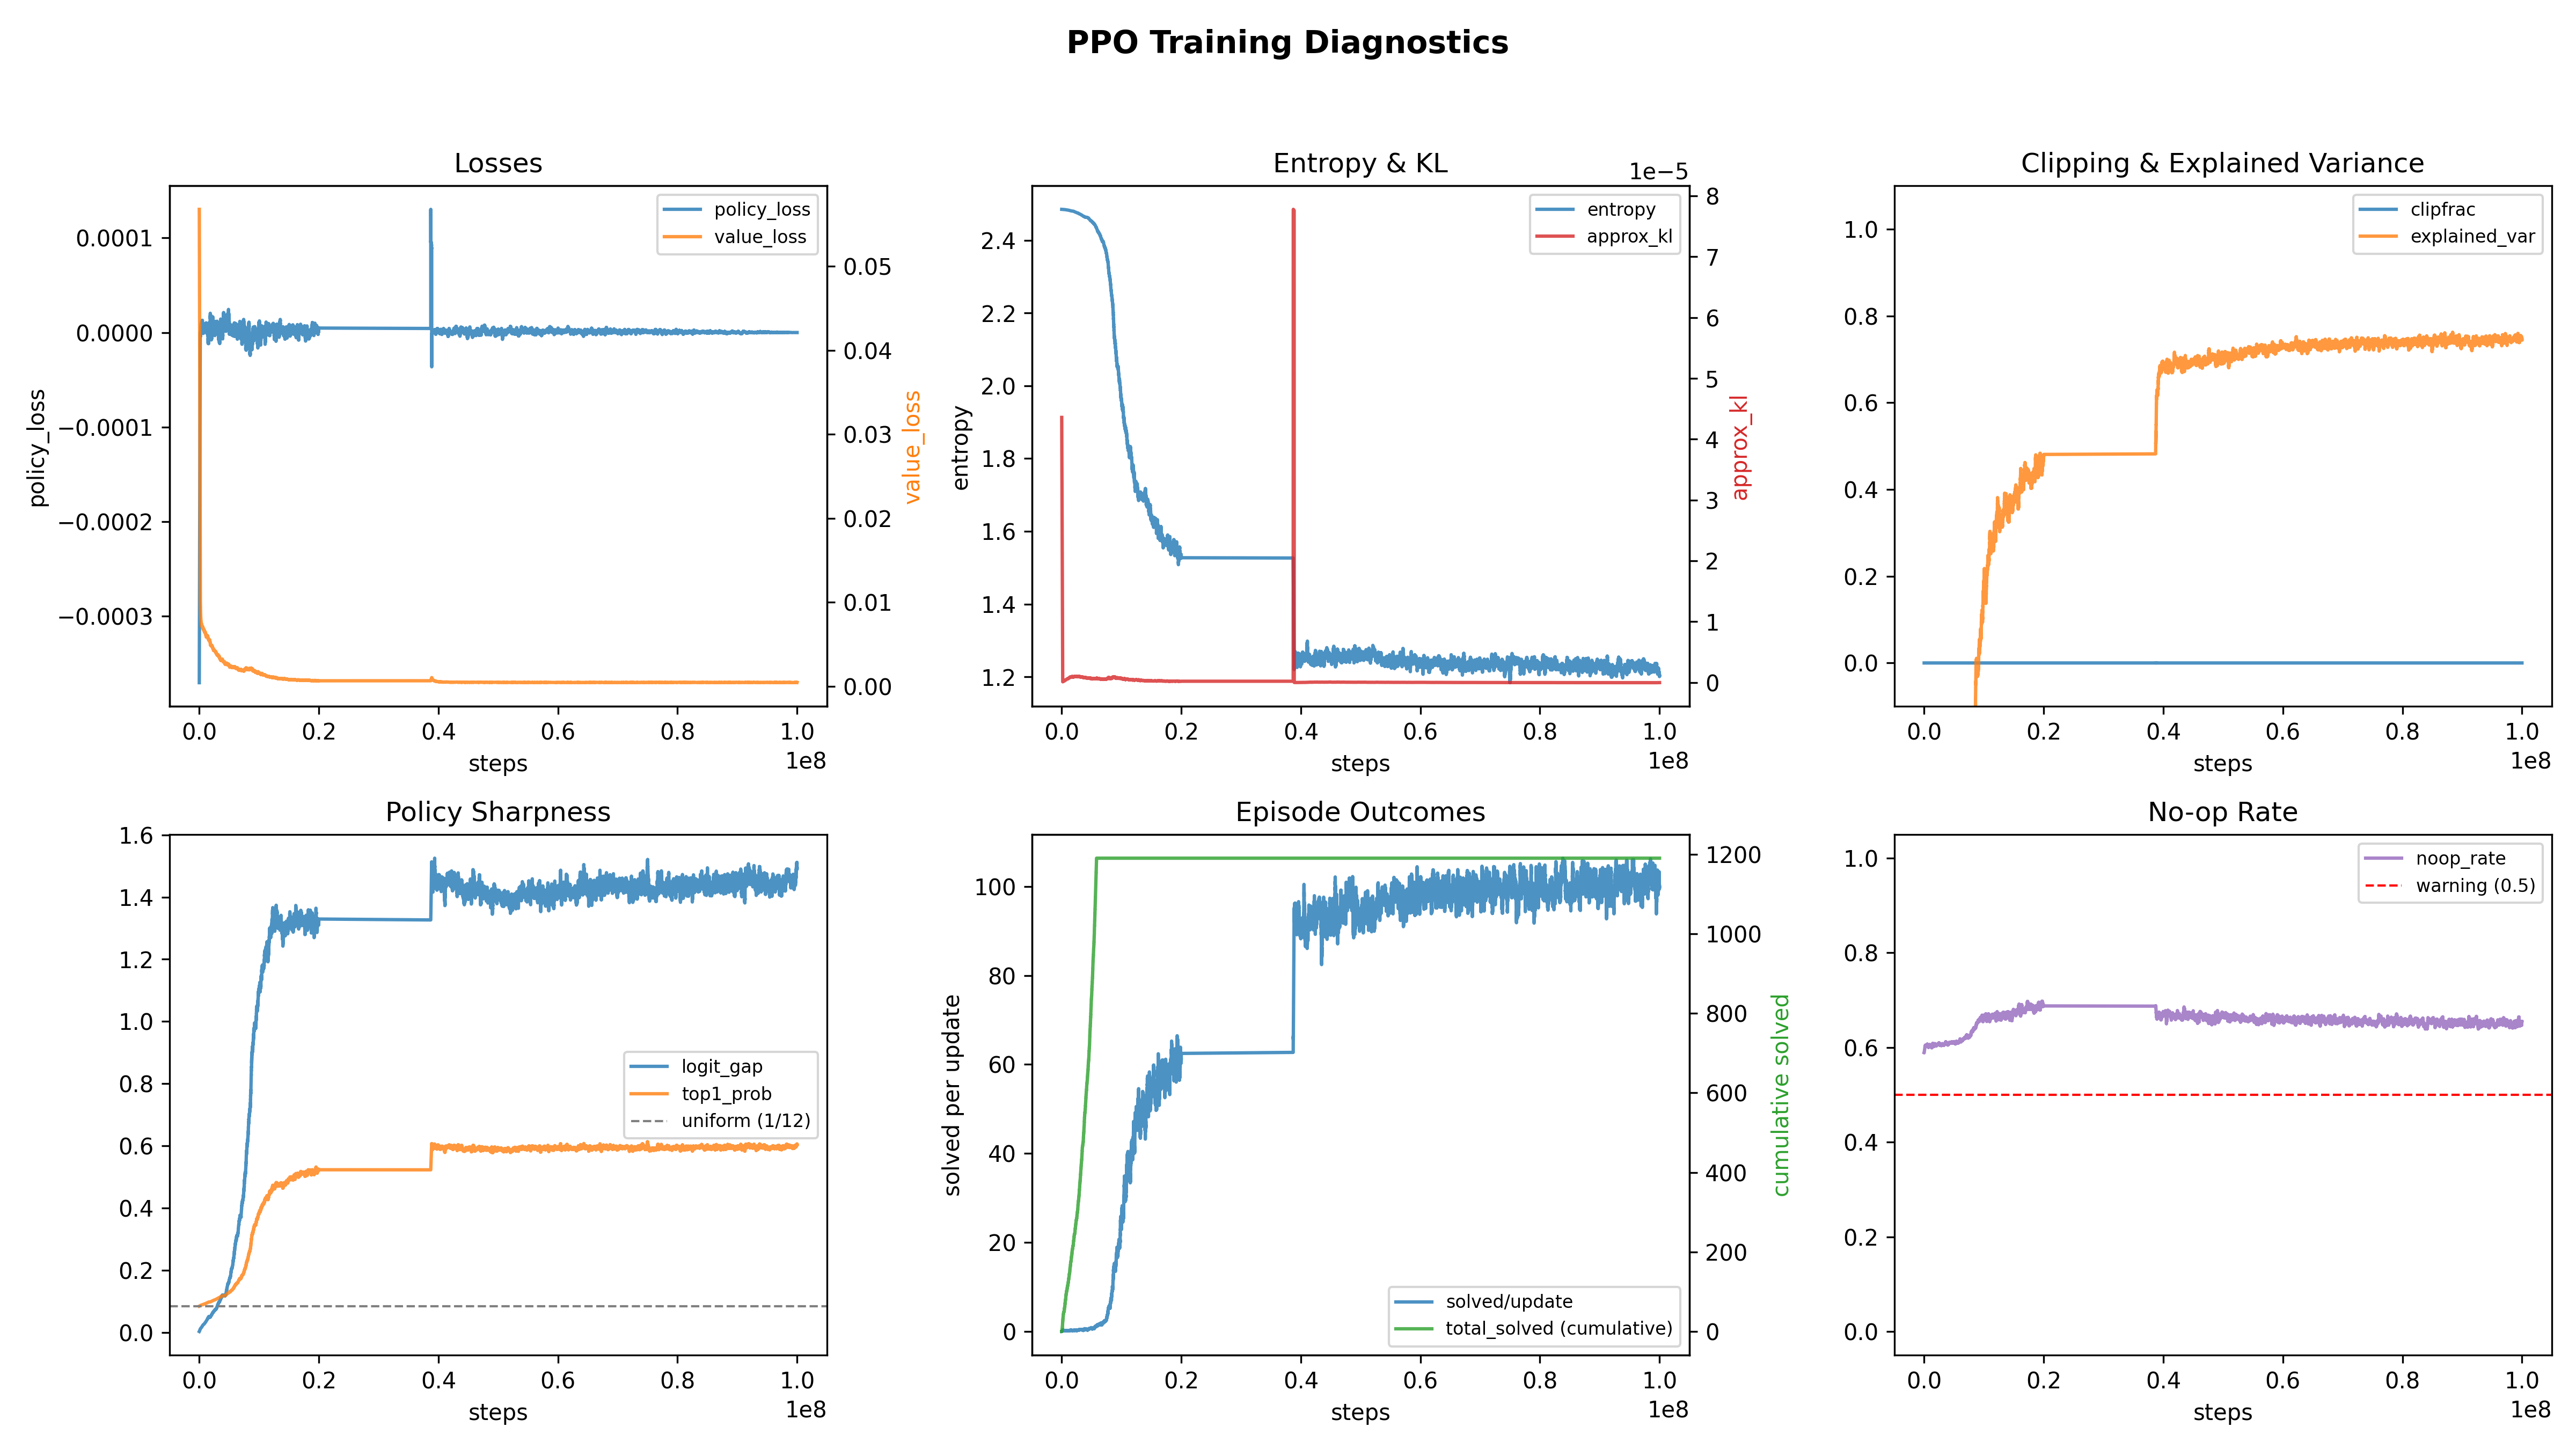
\includegraphics[width=0.95\textwidth]{figures/training_diagnostics.png}
  \end{center}
  \vspace{-0.5em}
  {\footnotesize \textbf{Top:} losses, entropy/KL, clipping/explained variance.
  \textbf{Bottom:} policy sharpness, episode outcomes, noop rate.}
\end{frame}

% ──────────────────────────────────────────────────────────────────────────────
\begin{frame}{Evidence of Learning}
  Four metrics confirm the network changed significantly:

  \bigskip
  \begin{center}
  \begin{tabular}{lrrl}
    \toprule
    \textbf{Metric} & \textbf{Start} & \textbf{End (100M)} & \textbf{Interpretation} \\
    \midrule
    Entropy     & 2.485 & 1.253 & Policy concentrates on subset \\
    Top-1 prob  & 8.4\% & 60.1\% & Strong action preference \\
    Logit gap   & 0.003 & 1.415 & Distinct preferences \\
    Expl.\ var  & $-0.92$ & $+0.66$ & Critic predicts success \\
    Clip frac   & 0.0   & 0.0   & Expected with epochs${}=1$ \\
    \bottomrule
  \end{tabular}
  \end{center}

  \bigskip
  \textbf{clipfrac $= 0$} is \textcolor{good}{expected}, not a bug---single epoch + tiny
  normalised advantages $\Rightarrow$ ratio stays within $[0.8, 1.2]$.
\end{frame}

% ──────────────────────────────────────────────────────────────────────────────
\begin{frame}{Action Distribution Shift}
  \begin{center}
    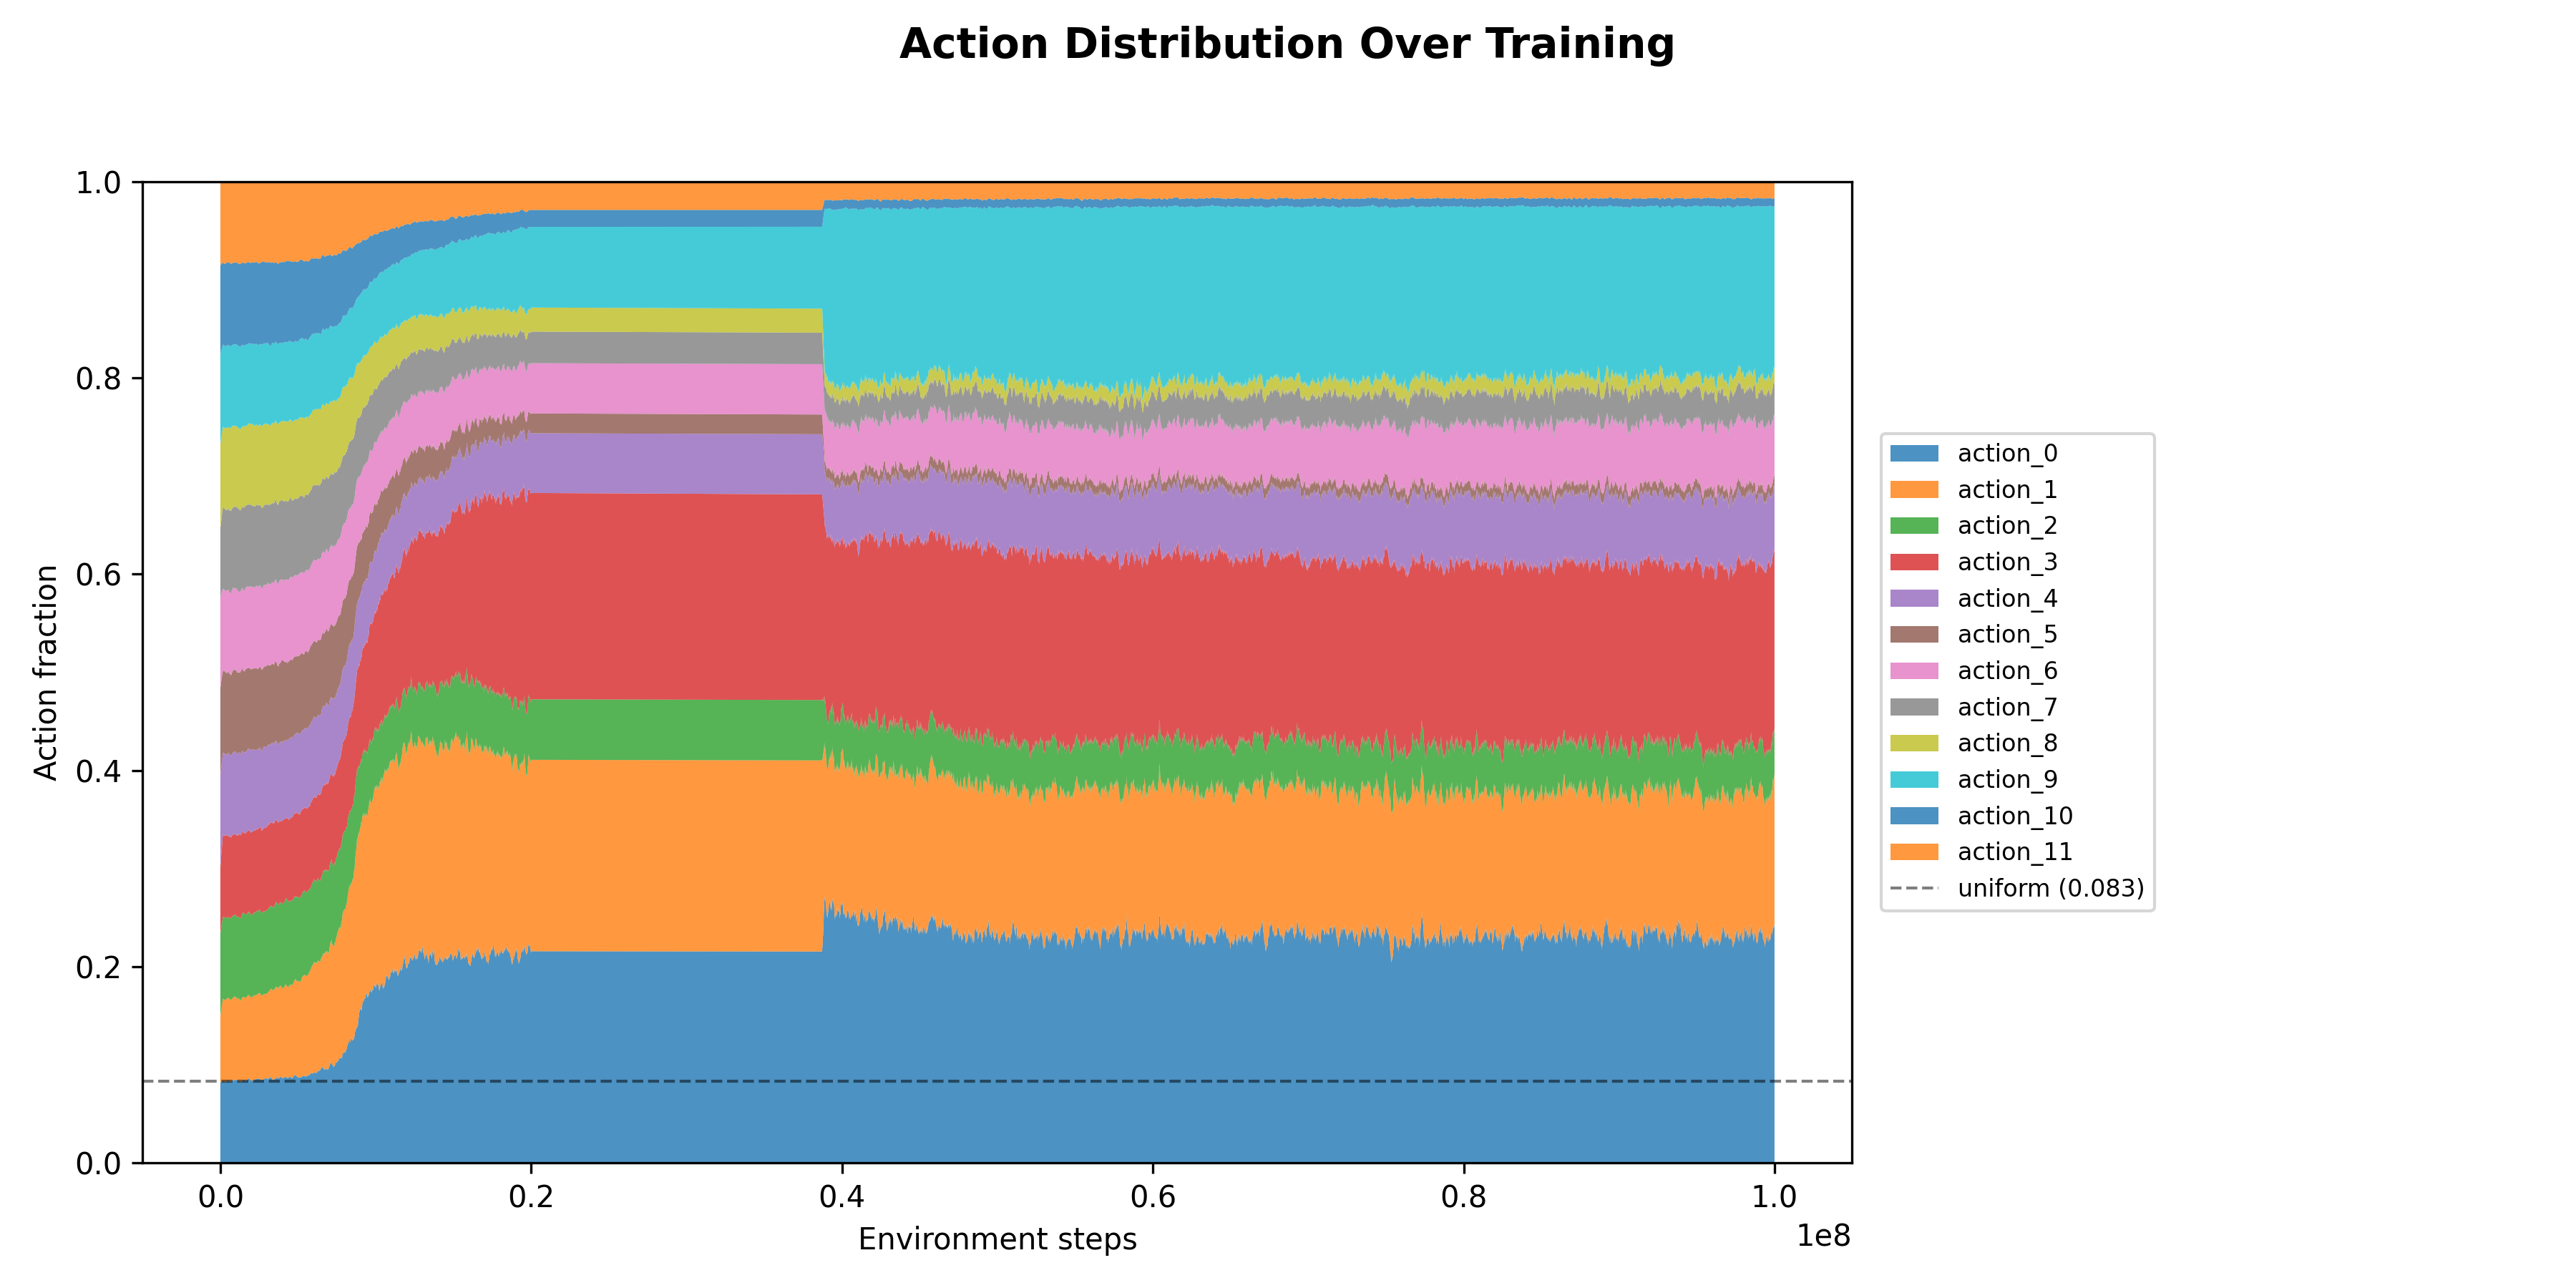
\includegraphics[width=0.75\textwidth]{figures/action_distribution.png}
  \end{center}
  \vspace{-0.5em}
  Policy shifts from uniform ($\sim$8.3\% each) to concentrated---favours
  \textbf{concatenations} (actions 0--3) over conjugations.
\end{frame}

% ──────────────────────────────────────────────────────────────────────────────
\begin{frame}{PPO Evaluation Results}
  \begin{center}
  \begin{tabular}{l@{\hskip 12pt}r@{\hskip 12pt}r@{\hskip 12pt}r}
    \toprule
    \textbf{Checkpoint} & \textbf{Greedy (det)} & \textbf{Stoch $\times$1} & \textbf{Stoch $\times$5} \\
    \midrule
    1M   & 0 (0.0\%)  & 2 (0.2\%)   & 7 (0.6\%)   \\
    5M   & 5 (0.4\%)  & 6 (0.5\%)   & 15 (1.3\%)  \\
    10M  & 7 (0.6\%)  & 12 (1.0\%)  & 30 (2.5\%)  \\
    20M  & 7 (0.6\%)  & 10 (0.8\%)  & 30 (2.5\%)  \\
    \rowcolor{highlight}
    \textbf{50M}  & \textbf{6 (0.5\%)}  & \textbf{16 (1.3\%)}  & \textbf{32 (2.7\%)} \\
    100M & 6 (0.5\%)  & 13 (1.1\%)  & 29 (2.4\%)  \\
    \bottomrule
  \end{tabular}
  \end{center}

  \bigskip
  \begin{itemize}
    \item \textbf{Peak at 50M}---LR$\to$0 schedule \textcolor{bad}{degraded} the policy after 50M
    \item All 1190 instances, horizon $= 200$
  \end{itemize}
\end{frame}

% ══════════════════════════════════════════════════════════════════════════════
\section{Comparative Analysis}
% ══════════════════════════════════════════════════════════════════════════════

% ──────────────────────────────────────────────────────────────────────────────
\begin{frame}{PPO vs.\ Classical Baselines}
  \begin{center}
  \begin{tabular}{lrr}
    \toprule
    \textbf{Algorithm} & \textbf{Solved} & \textbf{Rate} \\
    \midrule
    Greedy search ($10^6$ nodes)     & \textbf{554} / 1190 & \textcolor{good}{\textbf{46.6\%}} \\
    BFS ($10^6$ nodes)               & 278 / 1190           & 23.4\% \\
    \midrule
    PPO 50M (greedy eval)            & 6 / 1190             & \textcolor{bad}{0.5\%} \\
    PPO 50M (best-of-5 stoch)        & 32 / 1190            & \textcolor{bad}{2.7\%} \\
    \bottomrule
  \end{tabular}
  \end{center}

  \bigskip
  \begin{center}
  \Large
  Classical greedy search is \textcolor{accent}{\textbf{$17\times$ better}}\\
  than the best PPO configuration.
  \end{center}
\end{frame}

% ──────────────────────────────────────────────────────────────────────────────
\begin{frame}{Did PPO Learn Anything?}
  Compare best PPO (50M sto5) vs.\ near-random (1M sto5):

  \begin{center}
  \begin{tabular}{lrl}
    \toprule
    \textbf{Policy} & \textbf{Solved} & \textbf{Interpretation} \\
    \midrule
    Near-random (1M) & 7 / 1190 (0.6\%) & Random walk baseline \\
    PPO 50M          & 32 / 1190 (2.7\%) & \textcolor{good}{$4.6\times$ improvement} \\
    \midrule
    Overlap          & 4   & Solved by both \\
    PPO-only         & 28  & \textcolor{good}{Genuine learning} \\
    Random-only      & 3   & Noise \\
    \bottomrule
  \end{tabular}
  \end{center}

  \bigskip
  \textbf{Verdict:} PPO learned \textit{genuine but shallow} problem structure.\\
  Solves only the easiest instances (short lengths, low $n$).
\end{frame}

% ──────────────────────────────────────────────────────────────────────────────
\begin{frame}{Training Solve Rate $\neq$ Evaluation Solve Rate}
  \begin{columns}[T]
    \begin{column}{0.48\textwidth}
      \textbf{Training:}
      \begin{itemize}
        \item 94.5\% solve rate
        \item 1190/1190 marked ``solved''
        \item Uses stochastic sampling
        \item 200-step random walk often finds easy solutions
      \end{itemize}
    \end{column}
    \begin{column}{0.48\textwidth}
      \textbf{Evaluation:}
      \begin{itemize}
        \item 0.5\% greedy solve rate
        \item 2.7\% best-of-5 stochastic
        \item Tests what policy \textit{actually learned}
        \item Near-random baseline: 0.6\%
      \end{itemize}
    \end{column}
  \end{columns}

  \bigskip
  \begin{center}
    \alert{Training solve rate is misleading}---dominated by stochastic\\
    exploration, not learned policy quality.
  \end{center}
\end{frame}

% ══════════════════════════════════════════════════════════════════════════════
\section{Diagnosis \& Recommendations}
% ══════════════════════════════════════════════════════════════════════════════

% ──────────────────────────────────────────────────────────────────────────────
\begin{frame}{Why PPO Underperformed}
  \begin{enumerate}
    \item \textbf{Catastrophic reward attenuation}\\
      Success signal: $+14{,}400 \to +0.069$ ($200\times$ reduction)

    \item \textbf{Insufficient data reuse} (\texttt{update\_epochs} $= 1$)\\
      Standard PPO uses 3--10 epochs per batch

    \item \textbf{Batch size $3.5\times$ too small}\\
      1{,}600 vs.\ paper's 5{,}600 $\Rightarrow$ noisier gradients

    \item \textbf{LR$\to$0 degradation}\\
      50M checkpoint outperforms 100M

    \item \textbf{High noop rate ($\sim$69\%)}\\
      Two-thirds of actions produce no state change
  \end{enumerate}
\end{frame}

% ──────────────────────────────────────────────────────────────────────────────
\begin{frame}{Recommended Next Steps}
  \begin{enumerate}
    \item \textcolor{accent}{\textbf{Fix reward scaling}}
      --- remove clip or use running normalisation\\
      {\small\textcolor{gray}{Highest expected impact: 200$\times$ more signal}}

    \item \textbf{Increase \texttt{update\_epochs} to 4}
      --- $4\times$ more learning per batch\\
      {\small\textcolor{gray}{\texttt{target\_kl} = 0.01 prevents overfitting}}

    \item \textbf{Increase \texttt{num\_envs}} to 16--28
      --- better gradient quality

    \item \textbf{Cosine LR with floor}
      --- \texttt{min\_lr\_frac} $= 0.1$ (maintain $10^{-5}$)

    \item \textbf{Action masking}
      --- prevent guaranteed no-op moves

    \item \textbf{Monitor greedy eval during training}
      --- ground-truth metric
  \end{enumerate}
\end{frame}

% ══════════════════════════════════════════════════════════════════════════════
\section{Conclusions}
% ══════════════════════════════════════════════════════════════════════════════

% ──────────────────────────────────────────────────────────────────────────────
\begin{frame}{Summary}
  \begin{columns}[T]
    \begin{column}{0.48\textwidth}
      \textbf{Classical Search}
      \begin{itemize}
        \item Greedy: \textcolor{good}{\textbf{554/1190 (46.6\%)}}
        \item BFS: 278/1190 (23.4\%)
        \item No training required
        \item BFS matches paper exactly
      \end{itemize}
    \end{column}
    \begin{column}{0.48\textwidth}
      \textbf{PPO (100M steps)}
      \begin{itemize}
        \item Best: \textcolor{bad}{\textbf{32/1190 (2.7\%)}}
        \item $4.6\times$ better than random
        \item $17\times$ worse than greedy
        \item Code correct; signal too weak
      \end{itemize}
    \end{column}
  \end{columns}

  \bigskip
  \begin{block}{Key Takeaway}
    The PPO implementation is mechanically correct and the policy learned genuine
    (but shallow) structure.  The primary bottleneck is reward signal attenuation
    ($200\times$), not a bug.  Classical search remains far superior.
  \end{block}
\end{frame}

% ══════════════════════════════════════════════════════════════════════════════
\appendix
% ══════════════════════════════════════════════════════════════════════════════

\begin{frame}[fragile]{Appendix: Reproduction Commands}
  \small
  \textbf{Classical search:}
  \begin{lstlisting}[language=bash]
python -m ac_solver.search.miller_schupp.evaluate \
    --search-fn greedy --max-nodes 1000000 --workers 4 --full
python -m ac_solver.search.miller_schupp.evaluate \
    --search-fn bfs --max-nodes 1000000 --workers 4 --full
  \end{lstlisting}

  \textbf{PPO training:}
  \begin{lstlisting}[language=bash]
python -m ac_solver.agents.ppo --preset paper_faithful_mac --seed 1
  \end{lstlisting}

  \textbf{PPO evaluation:}
  \begin{lstlisting}[language=bash]
python -m ac_solver.agents.evaluate \
    --checkpoint out/<run>/ckpt_50000000.pt \
    --horizon 200 --full --stochastic --num-rollouts 5
  \end{lstlisting}
\end{frame}

% ──────────────────────────────────────────────────────────────────────────────
\begin{frame}{Appendix: Full Hyperparameter Table}
  \scriptsize
  \begin{center}
  \begin{tabular}{lrrl}
    \toprule
    \textbf{Parameter} & \textbf{Paper} & \textbf{Mac} & \textbf{Notes} \\
    \midrule
    \texttt{total\_timesteps}    & $10^8$  & $10^8$  & Same \\
    \texttt{num\_envs}           & 28      & 8       & Hardware \\
    \texttt{num\_steps}          & 200     & 200     & Episode horizon \\
    \texttt{batch\_size}         & 5{,}600 & 1{,}600 & $\text{envs} \times \text{steps}$ \\
    \texttt{minibatch\_size}     & 1{,}400 & 400     & batch / 4 \\
    \texttt{update\_epochs}      & 1       & 1       & \\
    LR                           & \multicolumn{2}{c}{$10^{-4} \to 0$} & Linear \\
    $\gamma$ / $\lambda_\text{GAE}$ & 0.999 / 0.95 & 0.999 / 0.95 & \\
    $\epsilon_\text{clip}$       & 0.2     & 0.2     & \\
    $c_\text{ent}$ / $c_\text{vf}$ & 0.01 / 0.5 & 0.01 / 0.5 & \\
    \texttt{max\_grad\_norm}     & 0.5     & 0.5     & \\
    KL target                    & 0.01    & 0.01    & Early stop \\
    \texttt{repeat\_solved\_prob}& 0.25    & 0.25    & Curriculum \\
    \midrule
    PPO updates                  & 17{,}857 & 62{,}500 & \\
    \bottomrule
  \end{tabular}
  \end{center}
\end{frame}

% ──────────────────────────────────────────────────────────────────────────────
\begin{frame}{Appendix: Metric Trajectory}
  \scriptsize
  \begin{center}
  \begin{tabular}{rrrrrrr}
    \toprule
    \textbf{Step} & \textbf{Entropy} & \textbf{Logit Gap} & \textbf{Top-1} & \textbf{Expl.\ Var} & \textbf{Clip} & \textbf{Solved} \\
    \midrule
    1.6K (start) & 2.485 & 0.003 & 0.084 & $-0.920$ & 0.0 & 0 \\
    1M    & 2.483 & 0.035 & 0.093 & $-2.062$ & 0.0 & 116 \\
    5M    & 2.454 & 0.172 & 0.130 & $-1.332$ & 0.0 & 843 \\
    10M   & 1.919 & 1.162 & 0.397 & $+0.397$ & 0.0 & 1190 \\
    20M   & 1.363 & 1.667 & 0.591 & $+0.510$ & 0.0 & 1190 \\
    50M   & $\sim$1.2 & $\sim$1.4 & $\sim$0.58 & $\sim$0.6 & 0.0 & 1190 \\
    100M  & 1.253 & 1.415 & 0.601 & $+0.656$ & 0.0 & 1190 \\
    \bottomrule
  \end{tabular}
  \end{center}

  \bigskip
  \small
  \begin{center}
  \begin{tabular}{lrrrrr}
    \toprule
    \textbf{Phase} & \textbf{Entropy} & \textbf{Top-1} & \textbf{Expl.\ Var} & \textbf{Noop} & \textbf{Solve \%} \\
    \midrule
    0--1M    & 2.484 & 0.089 & $-1.832$ & 0.604 & 2.5\% \\
    5--10M   & 2.283 & 0.229 & $-0.559$ & 0.632 & 49.3\% \\
    50--100M & 1.235 & 0.594 & $+0.734$ & 0.656 & 94.5\% \\
    \bottomrule
  \end{tabular}
  \end{center}
\end{frame}

\end{document}
